\documentclass[a4paper,12pt]{article}
\usepackage[top = 2.5cm, bottom = 2.5cm, left = 2.5cm, right = 2.5cm]{geometry}
\usepackage[T1]{fontenc}
\usepackage[utf8]{inputenc}
\usepackage{multirow} 
\usepackage{booktabs} 
\usepackage{graphicx}
\usepackage[spanish]{babel}
\usepackage{setspace}
\setlength{\parindent}{0in}
\usepackage{float}
\usepackage{fancyhdr}
\usepackage{amsmath}
\usepackage{amssymb}
\usepackage{amsthm}
\usepackage[numbers]{natbib}
\newcommand\Mycite[1]{%
	\citeauthor{#1}~[\citeyear{#1}]}
\usepackage{graphicx}
\usepackage{subcaption}
\usepackage{booktabs}
\usepackage{etoolbox}
\usepackage{minibox}
\usepackage{hyperref}
\usepackage{xcolor}
\usepackage{pdfpages}
\usepackage[skins]{tcolorbox}
%---------------------------

\newtcolorbox{cajita}[1][]{
	 #1
}

\newenvironment{sol}
{\renewcommand\qedsymbol{$\square$}\begin{proof}[\textbf{Solución.}]}
	{\end{proof}}

\newenvironment{dem}
{\renewcommand\qedsymbol{$\blacksquare$}\begin{proof}[\textbf{Demostración.}]}
	{\end{proof}}

\newtheorem{problema}{Problema}
\newtheorem{definicion}{Definición}
\newtheorem{ejemplo}{Ejemplo}
\newtheorem{teorema}{Teorema}
\newtheorem{corolario}{Corolario}[teorema]
\newtheorem{lema}[teorema]{Lema}
\newtheorem{prop}{Proposición}
\newtheorem*{nota}{\textbf{NOTA}}
\renewcommand\qedsymbol{$\blacksquare$}
\usepackage{svg}
\usepackage{tikz}
\usepackage[framemethod=default]{mdframed}
\global\mdfdefinestyle{exampledefault}{%
linecolor=lightgray,linewidth=1pt,%
leftmargin=1cm,rightmargin=1cm,
}




\newenvironment{noter}[1]{%
\mdfsetup{%
frametitle={\tikz\node[fill=white,rectangle,inner sep=0pt,outer sep=0pt]{#1};},
frametitleaboveskip=-0.5\ht\strutbox,
frametitlealignment=\raggedright
}%
\begin{mdframed}[style=exampledefault]
}{\end{mdframed}}
\newcommand{\linea}{\noindent\rule{\textwidth}{3pt}}
\newcommand{\linita}{\noindent\rule{\textwidth}{1pt}}

\AtBeginEnvironment{align}{\setcounter{equation}{0}}
\pagestyle{fancy}

\fancyhf{}









%----------------------------------------------------------
\lhead{\footnotesize Data Science I}
\rhead{\footnotesize  Rudik Roberto Rompich}
\cfoot{\footnotesize \thepage}


%--------------------------

\begin{document}
 \thispagestyle{empty} 
    \begin{tabular}{p{15.5cm}}
    \begin{tabbing}
    \textbf{Universidad del Valle de Guatemala} \\
    Departamento de Ciencias de la Computación\\\\
   \textbf{Estudiantes:} Augusto Alonso, Angel Cuellar, Rudik Roberto Rompich\\
    \end{tabbing}
    \begin{center}
        CC3066 - Data Science I - Catedrático: Luis Furlan\\
        \today
    \end{center}\\
    \hline
    \\
    \end{tabular} 
    \vspace*{0.3cm} 
    \begin{center} 
    {\Large \bf  Proyecto 2 - Análisis Exploratorio 
} 
        \vspace{2mm}
    \end{center}
    \vspace{0.4cm}
%--------------------------

\textbf{Instrucciones:} en clase vimos un modelo simple para resolver regresiones lineales mediante redes neuronales.  Utilizado el código desarrollado (o si lo desea uno propio), responda a las siguientes preguntas:

\begin{cajita}
	Para realizar este laboratorio se hicieron algunas modificaciones al código proporcionado por el catedrático: 
	\begin{enumerate}
		\item Se utilizó \textit{seaborn} en lugar de \textit{plotly}, debido a que las gráficas ya no se generaban cuando las observaciones eran demasiado grandes. 
		\item Para determinar los tiempos de ejecución, \textbf{no se corrieron las gráficas} (ya que es la parte del código que consume más tiempo) y lo importante son los 3 datos que se obtuvieron. 
		\item Se modificaron las iteraciones y se colocaron 6000 con un $\eta= $0.1 (eta); ya que con ese número en todos los casos daba los números esperados (y no era necesario correr varias veces la celda anterior, como se indicaba en las instrucciones).
		\item Para medir el tiempo de ejecución se utilizó la librería de \textit{time}.  
	\end{enumerate}
\end{cajita}

\begin{problema}
	Cambie el número de observaciones a 100,000.  Explique que es lo que ocurre en términos de:
	\begin{enumerate}
		\item El tiempo de ejecución para resolver el problema.
		\begin{sol}
			El tiempo de ejecución en segundos es un poco más prolongado; pero no excesivamente, alrededor de 9 segundos.			\begin{figure}[H]
				\centering
				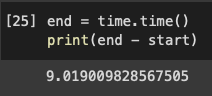
\includegraphics[scale=0.5]{Images/1.3}
			\end{figure}
		\end{sol}
		\item El resultado final versus lo encontrado en clase:  es igual, o diferente...¿por qué?
		\begin{sol}
				Es prácticamente igual, mismos pesos y sesgo. 
			\begin{figure}[H]
				\centering
				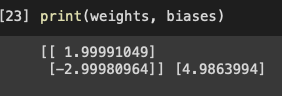
\includegraphics[scale=0.5]{Images/1.4}
			\end{figure}
		\end{sol}
		\item Las gráficas  para representar los datos/resultados.
		\begin{sol}
			Las gráficas con 100,000 observaciones no varían en prácticamente nada la forma con las 1000 iteraciones iniciales. 
			\begin{figure}[H]
				\centering
				\begin{subfigure}{.5\textwidth}
					\centering
					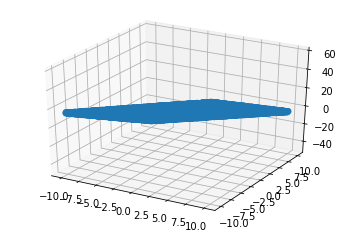
\includegraphics[width=0.45\textwidth]{Images/1.1}
				\end{subfigure}%
				\begin{subfigure}{.5\textwidth}
					\centering
					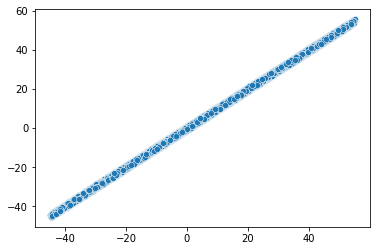
\includegraphics[width=0.45\textwidth]{Images/1.2}
				\end{subfigure}
			\end{figure}
		\end{sol}
	\end{enumerate}
\end{problema}

\begin{problema}
	Cambie el número de observaciones a 1,000,000.  Explique que es lo que ocurre en términos de:
		\begin{enumerate}
		\item El tiempo de ejecución para resolver el problema.
		\begin{sol}
			El tiempo de ejecución en segundos es relativamente grande, rondando en alrededor de los 2 minutos de tiempo de ejecución (esto influyó por el número de iteraciones).
			\begin{figure}[H]
				\centering
				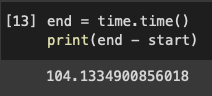
\includegraphics[scale=0.5]{Images/2.3}
			\end{figure}
		\end{sol}
		\item El resultado final versus lo encontrado en clase:  es igual, o diferente...¿por qué?
		\begin{sol}
			El resultado es prácticamente igual, mismos pesos y sesgo. 
			\begin{figure}[H]
				\centering
				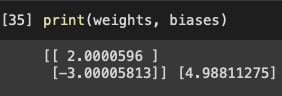
\includegraphics[scale=0.5]{Images/2.4}
			\end{figure}
		\end{sol}
		\item Las gráficas  para representar los datos/resultados.
		\begin{sol}
			Las gráficas con 1,000,000 observaciones no varía en absolutamente nada comparado a las 100,000 y 1000 observaciones. Quizás simplemente son más robustas. 
			\begin{figure}[H]
				\centering
				\begin{subfigure}{.5\textwidth}
					\centering
					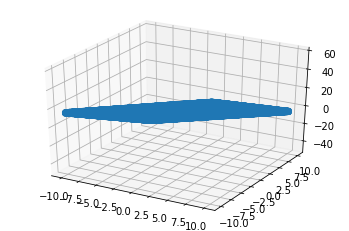
\includegraphics[width=0.45\textwidth]{Images/2.1}
				\end{subfigure}%
				\begin{subfigure}{.5\textwidth}
					\centering
					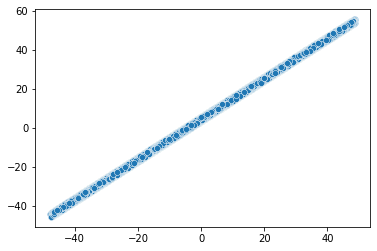
\includegraphics[width=0.45\textwidth]{Images/2.2}
				\end{subfigure}
			\end{figure}
		\end{sol}
	\end{enumerate}

\end{problema}

\begin{problema}
	“Juegue” un poco con el valor de la tasa de aprendizaje, por ejemplo  0.0001, 0.001, 0.1, 1.  Para cada uno de estos indique:
	\begin{enumerate}
		\item ¿Qué ocurre con el tiempo de ejecución?
		\begin{sol}
			El tiempo de ejecución va aumento cuando el $\eta$ va aumentando, por lo tanto es directamente proporcional. 
		\end{sol}
		\item ¿Qué ocurre con la minimización de la pérdida?
		\begin{sol}
			En los primeros dos casos, la pérdida va disminuyendo. Sin embargo, para los últimos dos casos la pérdida se vuelve increíblemente grande.
		\end{sol}
		\item ¿Qué ocurre con los pesos y los sesgos?
			\begin{sol}
			En todos los casos los pesos son iguales; únicamente el sesgo varía drásticamente. 
		\end{sol}
		\item ¿Qué ocurre con las iteraciones?
			\begin{sol}
			Se utilizaron 6000 iteraciones en todos los casos, ya que en la pregunta 1 y 2 se determinó que era el número ideal para encontrar los pesos y sesgo correcto. 
		\end{sol}
		\item ¿El problema queda resuelto o no?  
			\begin{sol}
			Sí, pero únicamente cuando el $\eta$ es pequeño. 
		\end{sol}
		\item ¿Cuál es la apariencia de la última gráfica?  ¿Se cumple con la condición de que sea de 45 grados?
			\begin{sol}
			No, la última gráfica explota en los últimos dos casos; ya que los números son demasiado grandes. 
		\end{sol}
	\end{enumerate}
	
\end{problema}

\begin{problema}
	Cambie la función de pérdida “L2-norm” a la misma pero sin dividir por 2.  Explique lo que ocurre en términos de:
	\begin{enumerate}
		\item El tiempo que se tarda el algoritmo en terminar, comparado a lo que vimos en clase.
		\begin{sol}
			El tiempo incrementa, aproximadamente el doble.
		\end{sol}
		\item Si la pérdida se minimiza igual que lo que vimos en clase.
		\begin{sol}
			En efecto, la pérdida se minimiza. 
		\end{sol}
		\item Si los pesos y sesgos son parecidos a los vistos en clase.
		\begin{sol}
			Sí, los pesos son los mismos; el sesgo varía un poco. 
		\end{sol}
		\item Si el problema se resuelve como ocurrió en clase.
		\begin{sol}
			Sí, el problema también se resolvió quitándole el 2. 
		\end{sol}
		\item Si se obtiene un mejor resultado al hacer más iteraciones.
		\begin{sol}
			Es una pregunta más o menos inconclusa; ya que al utilizar más iteraciones se obtiene el sesgo correcto un poquito más antes. 
		\end{sol}
	\end{enumerate}
\end{problema}

\begin{problema}
	Cambie la función de pérdida de la “L2-norm” a la “L1-norm”.  Explique lo que ocurre en términos de:
	
	\begin{enumerate}
		\item El tiempo que se tarda el algoritmo en terminar, comparado a lo que vimos en clase
		\begin{sol}
			Levemente más alto, alrededor de 1 segundo más tardado. 
		\end{sol}
		\item Si la pérdida se minimiza igual que lo que vimos en clase
		\begin{sol}
			No, ahora va de un número negativo hasta llevar a acercarse a 0. 
		\end{sol}
		\item Si los pesos y sesgos son parecidos a los vistos en clase
		\begin{sol}
			Sí, son similares nuevamente los pesos; únicamente el sesgo varía. 
		\end{sol}
		\item Si el problema se resuelve como ocurrió en clase
		\begin{sol}
			Sí, el problema igualmente se resolvió.
		\end{sol}
		 \item Si se obtiene un mejor resultado al hacer más iteraciones.
		 \begin{sol}
		 	Así es, a más iteraciones; mejor resultado. El número de iteraciones propuesto es de 6000. 
		 \end{sol}
		 \item  ¿Tendrá una de estas más limitaciones que la otra? 
		 \begin{sol}
		 	Es probable que su límitante sea el tiempo.
		 \end{sol}
	\end{enumerate}
\end{problema}

\begin{problema}
	Cree una función $f(x,z) = 13 * x_s + 7 * z_s  - 12$. 
	\begin{enumerate}
		\item ¿Funciona el algoritmo de la misma forma?
		\begin{sol}
			Se modificó el código con la siguiente celda:
				\begin{figure}[H]
				\centering
				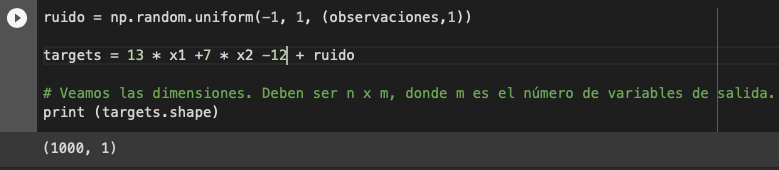
\includegraphics[scale=0.5]{Images/3}
			\end{figure}
		En conclusión, el algoritmo funciona de la misma manera, ya que solo se está modificando el \textit{target}; pero todo lo demás funciona exactamente igual. 
		\end{sol}
	\end{enumerate}
	
\end{problema}



%---------------------------

\end{document}